\chapter{LHC and ATLAS}
\label{sec:LHCandATLAS}
The data used in this thesis comes from the Atlas experiment at LHC. In this chapter,  a brief introduction to both the experiment and the accelerator will be presented. We will also get a small incite to the organization behind the experiment and the accelerator, namely CERN. 

\section{CERN}
\label{sec:cern}

The European organisation for nuclear research, CERN, started as a research facility on mainly nuclear physics. It was built on the border between France and Switzerland near Geneva in 1954. CERN have 22 member states, where Norway is one of the founding members, but it welcomes people from all over the world to take part in the different experiments and accelerator development. 

CERN quickly became the biggest and leading research centre in particle physics as well, and the most famous discoveries done at CERN are the discoveries done with high energy particle collisions. To mention some of the discoveries done at CERN we have weak neutral currents that are mediated by the hypothetical Z-boson in 1973 \cite{Zmed} and of course the discovery of the actual Z-boson and the W-boson mediators of the weak force in 1983/84 \cite{WZ1, WZ2, WZ3}. The most recent discovery is certainly that of the Higgs boson \cite{Higgs_ATLAS, Higgs_CMS} in 2012 by the ATLAS and CMS experiments, which also was the last piece to confirm the SM.

Through out the years there have been built many different accelerators at CERN. Among others the Super Proton Synchrotron (SPS) accelerated protons and antiprotons and allowed the UA1 and UA2 experiments to discover the Z- and W-bosons. The Large electron positron collider (LEP) was built in a 27 km long tunnel 100 m below ground and was definitively the biggest accelerator at the time. LEP allowed important SM precision measurements. The last run at LEP was done in 2000 paving the road for the start of building the Large Hadron Collider (LHC) which is the accelerator that produced proton-proton collisions data recorded by the ATLAS detector and which have been used to obtain the data for this thesis. 

\section{LHC - Large Hadron Collider}
\label{sec:LHC}

The Large Hadron Collider (LHC) \cite{LHCcern} is a 27km long particle accelerator 100 meters below ground and it is the most powerful of its kind in the world. Since LHC replaced LEP, the tunnel already existed which made the building a bit less comprehensive. The collider consists of superconducting magnets with accelerating structures to boost the proton velocity close to the speed of light, in an environment cooled down to 1.85K (-271.3$^o$C) to insure superconductivity. The LHC collider is shown in figure \ref{fig:LHC} as part of a complex of CERN accelerators. 

\begin{figure}[H]
    \centering
    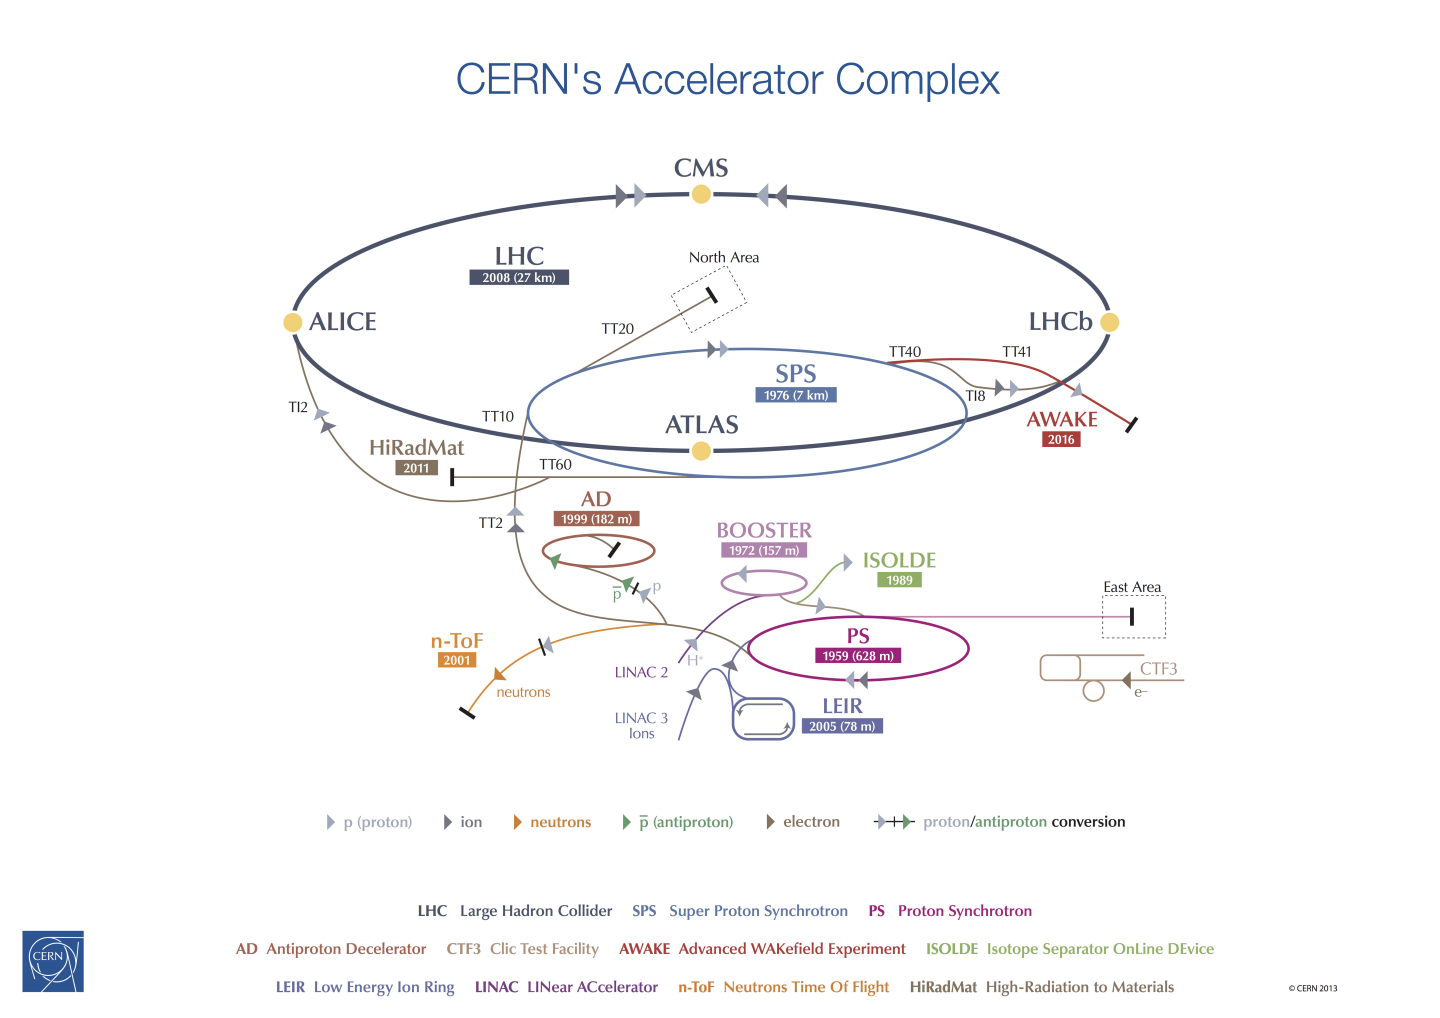
\includegraphics[width=\textwidth]{Figures/FromOnline/Poster-2013-377.jpg}
    \caption{An illustration of the accelerator complex at CERN \cite{LHCpic}}
    \label{fig:LHC}
\end{figure}

The protons extracted from a hydrogen bottle go through smaller accelerators to gain more energy before they in the end are sent in opposite directions into the LHC which is the big circle we can see in figure \ref{fig:LHC}. The particles get accelerated to about 99.99\% of the speed of light and a maximum energy of 6.5 TeV. In the end the two beams of protons will collide in the centre of four experiments around LHC, which are marked with yellow dots in figure \ref{fig:LHC}, namely ATLAS, ALICE, CMS and LHCb. 

The different experiments focus on different research goals. ATLAS (A Toridal LHC ApparatuS) and CMS (Compact
Muon Solenoid) are multipurpose detectors mainly focusing on SM measurements and searches for new physics, i.e. discovery of new particles and phenomena, e.g. SUSY. The last big achievement of ATLAS and CMS is the discovery of the Higgs boson. While ALICE (A Large Ion Collider Experiment) focuses on heavy ion collisions with lead-lead and lead-proton to study the quark-gluon plasma, LHCb (Large Hadron Collider beaty) focuses on processes related to b-quarks to precisely measure CP violation and oscillation phenomena. 

At the LHC we focus on proton-proton collisions (and heavy ion collisions) to study various high energy final states via electroweak and strong interactions with the hope to discover new phenomena. The internal structure of the proton allows to register a large amount of events in a single collision and thus collect a wider statistics for our experiments. The number of collisons per area per second is defined thorugh the luminosity $\mathscr{L}$, given by

\begin{equation}
    \label{eq:lumi}
    \mathscr{L} = f \frac{n_1 n_2}{4 \pi \sigma_x \sigma_y},
\end{equation}

where f is the crossing rate of the proton bunches, $n_i$ is the number of colliding particles in each bunch and $\sigma_{x,y}$ is the spread of the bunch along the x- and y-direction.  

Using the integrated luminsoty over time we can find the number of interactions $N$ in our dataset. This is given by  
\begin{equation}
    \label{eq:intLumi}
    N = \sigma \int \mathscr{L}(t) dt, 
\end{equation}

where $\sigma$ is the cross section for a certain process. 

As the luminosity gets higher, we have more collisions happening in the detector. This gives us a lot of interactions at the same time, which can introduce further systematic uncertainty. This phenomenon is called \textit{pile-up}. We need to consider this to know which particles in the final state comes from which interaction. This is a constantly evolving problem since we are further developing the LHC infrastructures and apparatus towards higher and higher luminosity, e.g. HL-LHC (High Luminosity LHC).








\section{The ATLAS detector}
\label{sec:ATLAS}
\begin{comment}


\begin{itemize}
    \item Skriv kort om ATLAS
    \item Tracking
    \item luminositet osv
    \item luminosity $10^{34} cm^{-2}s^{-1}$ for proton-proton
    \item upgrade to HL-LHC
    \item size
    \item figure of tracks
    \item coordinate system and navngiving og nyttige variabler: lumi og pileup og number of interations and rate.
    \item origin of the coordinate system: nominal interaction point
    \item $\phi$ og $\Theta$
    \item transverse og alle er definert i x-y-planet
    \item pseudo rapidity
    \item $\Delta R_{ll}$
    \item INNER DETECTOR:
    \item Hvor den er
    \item Exposed for mye radiation og derfor må vi oppgradere nå
    \item scheduled at 2024, men vil bli utsatt (som er neste oppgradering igjen)
    \item Tracker de første bevegelsene av partiklene som er skapt i kollisjonen og må være veldig presis. 
    \item inner detector er inni et 2T magnetfelt som kommer fra the central solenoid. Som er med på å hjelpe oss å tracke partikler fordi ladde partikler vil bendes av mahnetfeltet.
    \item bilde av inner detector
    \item CALORIMETERS:
    \item Du må vite energien for å rekonsturere partikler fra kollisjonen. Calorimeteret måler hvor mye energi partikkelen legger igjen når den møter detektormaterialet.
    \item To er brukt: one EM calorimeter og hadronic calorimeter
    \item Bilde av begge calorimeters (en figur)
    \item Vi trenger calorimeters for å tracke ET og det er viktig for BSM.
    \item EM cal:
    \item for å tracke electrons og photons 
    \item HAD cal:
    \item Outside of EM og den er bygd for å tracke hadrons og hadronic showers. Legg in hva en shower er. cascade decay.
    \item jet reconstruction og met
    \item MAGNETS:
    \item ATLAS består av to magnetsystemer: a central solenoid og a barrel (symmetrisk rundt beam axis) toreoid og two end-cap toreoids. 
    \item MUON system:
    \item basert på magnet deflection of muon tracks. Muon kammerne eksisterer rundt hele detektoren hvor den går rundt beam aksen og de ytterste ligger i x-y-planet. Ligger som en tønne rundt beam aksen og med lokk på endene. barrel region og end-cap regions.
    \item Triggers and data acquesition? 
    
\end{itemize}
\end{comment}
The ATLAS \cite{ATLAS} detector is a massive 44 m long detector, 25 m in diameter and weighing about the same as the Eiffel tower ($\sim 7000$ tons). It is designed to handle proton-proton collisions up to 14 TeV with a luminosity of a few times $10^{34}$cm$^{-2}$s$^{-1}$. We can see an illustration of the whole detector in figure \ref{fig:atlas}, where the most important components are marked. 


\begin{figure}[H]
    \centering
    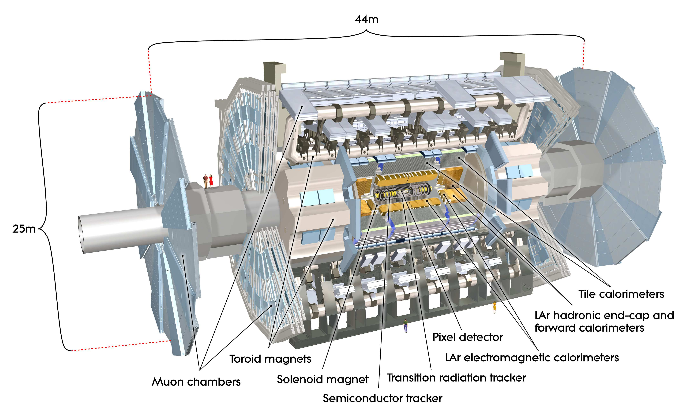
\includegraphics[width = \textwidth]{Figures/FromOnline/ATLAS.png}
    \caption{An illustration of the ATLAS detector \cite{ATLAS}.}
    \label{fig:atlas}
\end{figure}

The detector is built up in three main layers. Two inner tracking layers, that provide the information about particle trajectories and allow to determine, with good resolution, the interaction point and secondary vertices. The inner detector is composed of a pixel and strip silicon tracker and a transition radiation tracker. A good tracking resolution is in fact needed for particle identification purposes: the whole inner detector is inserted in a solenoid magnet that generates a magnetic field along the beam direction. The bending trajectory of charged particles in magnetic field leads to a determination of momentum and electric charge of the particles.

The tracker is followed by two layers of calorimeters. The innermost is the electromagnetic calorimeter and consists of alternating layers of lead and liquid argon. The purpose of the layer is to stop photons, positrons and electrons by inducing electromagnetic showers that allow to measure the energy of the particles. The outer calorimeter is the hadronic calorimeter, composed of three different detectors. The hadrons produced in the event interact with the calorimeter material and produce hadronic showers, also called \textit{jets}, that lose their whole energy in this layer. 

The outer layer consists of the muon chambers, which surround the whole detector as a barrel with two end-caps at the edges. Muons are the only detectable particles that are able to travel through all the other layers, only depositing a minimum ionisation energy. 

All the particles we cannot track in the detector layers are referred to as missing energy/momentum, essentially inferred from energy-momentum conservation and the measurement of all visible particles the energy difference $E_{miss} = -\sum_i E_i$ and $\Vec{p}_{miss} = -\sum_i \Vec{p}_i$. 

A sketch of the layers presented above is shown in figure \ref{fig:tracks}.

\begin{figure}[H]
    \centering
    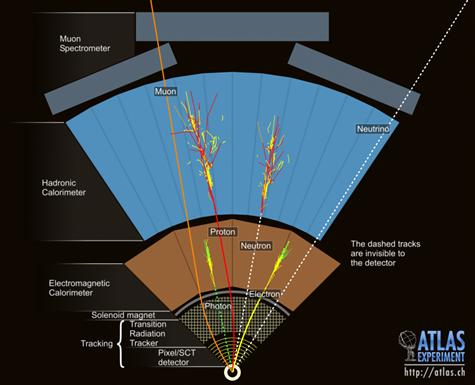
\includegraphics[width = 0.8\textwidth]{Figures/FromOnline/tracks.jpg}
    \caption{An illustration on how we see the tracks of the different particles in the detector \cite{tracks}.}
    \label{fig:tracks}
\end{figure}


\subsection{Variables and coordinates}
Combining information from the different layers it is possible to calculate different variables and identify the different particle species. We have two particles with opposite momentum $p$ in each collision and therefore we are interested only in the transverse direction, since the longitudinal momentum of the final states is negligible at such high energies. The energy deposited by the particle is measured by the detector and combined with the tracking information to have the vector quantities of $p_T$ and $E_T$ connected by the invariant mass m of the particle by the relation $p_T^2 = E_T^2 - m^2$. As mentioned before we can measure the energy difference between before and after the collision that gives us the \textit{missing transverse energy} (MET/$E_T^{miss}$). 

It is also useful to introduce the coordinates used within the detector to describe an event. A sketch is shown in figure \ref{fig:coordsys}. The $z$-coordinate is defined by the beam direction and the $x,y$-coordinates define the transverse plane. In addition we have the two angles $\theta$ and $\phi$, respectively the angle between the particle and the $z$-axis and the one with respect to the $x$-axis. Note that instead of referring to the coordinate $\theta$ it is common to introduce the pseudorapidity $\eta$ defined as 

\begin{equation}
    \eta = -\ln \tan \bigg(\frac{\theta}{2}\bigg).
\end{equation}

\begin{figure}[H]
    \centering
    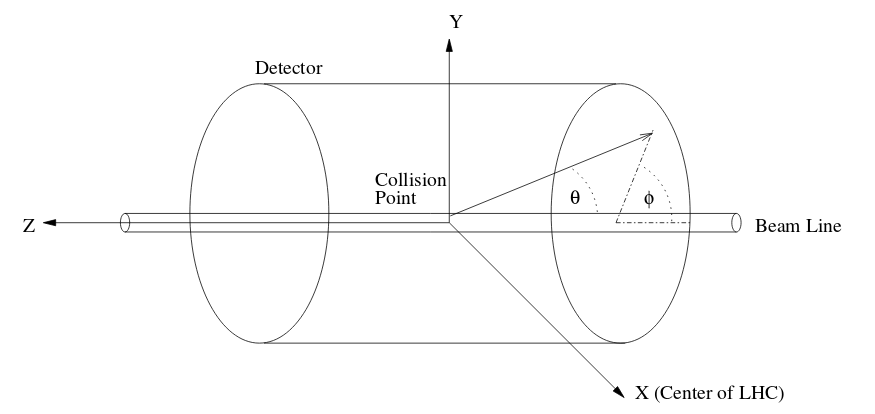
\includegraphics[width = \textwidth]{Figures/FromOnline/coordinatesystem.png}
    \caption{An illustration of the coordinate system inside the detector\cite{coordinatesystem}.}
    \label{fig:coordsys}
\end{figure}

The other variables we are considering in this thesis are listed below

\begin{itemize}
    \item $m_{l^+l^-}$ is the invariant mass of the lepton pair in the final state, defined as 
            \begin{equation}
                m_{l^+l^-} = \sqrt{(E_{l^+} + E_{l^-})^2 - (\mathbf{p}_{l^+} + \mathbf{p}_{l^-})^2}.
            \end{equation}
    \item $m_{T2}$ is the stransverse mass \cite{sleptonexclusion} and is used to describe the masses of a particle pair that is assumed to have decayed to one visible and one invisible particle. It is defined as 
    \begin{equation*}
        m_{T2}(\mathbf{p}_{T,1}, \mathbf{p}_{T,2}, \mathbf{p}_{T}^{miss}) = \min_{q_{T,1} + q_{T,2} = p_T^{miss}} \bigg\{\max\big[m_T(\mathbf{p}_{T,1}, \mathbf{q}_{T,1}), m_T(\mathbf{p}_{T,2}, \mathbf{q}_{T,2})\big]\bigg\},
    \end{equation*}
    where $m_T$ is the transverse mass (defined as $m_T = \sqrt{2 |\mathbf{p}_{T,1}| \cdot |\mathbf{p}_{T,2}| \cdot \big(1-\cos(\Delta\phi)\big)}$), $\mathbf{p}_{T,1}$ and $\mathbf{p}_{T,2}$ are the transverse momentum vectors of the two leptons in the final state, and $\mathbf{q}_{T,1}$ and $\mathbf{q}_{T,2}$ are vectors with $\mathbf{p}_{T}^{miss} = \mathbf{q}_{T,1} + \mathbf{q}_{T,2}$. 
    \item  $H_T$ is the scalar sum of the $p_T$ of the jets and leptons we have selected.
    \item  $\Delta \phi (\Vec{p}_T^{ll}, E_T^{miss})$ is the azimuthal angle difference between the two lepton system and the missing transverse energy.
    \item $\Delta R_{ll} = \sqrt{(\Delta\phi_{ll})^2 + (\Delta \eta_{ll})^2}$ is the distance between the two leptons in the final state.
\end{itemize}


   
  
    







\begin{comment}


\begin{figure}[H]
    \centering
    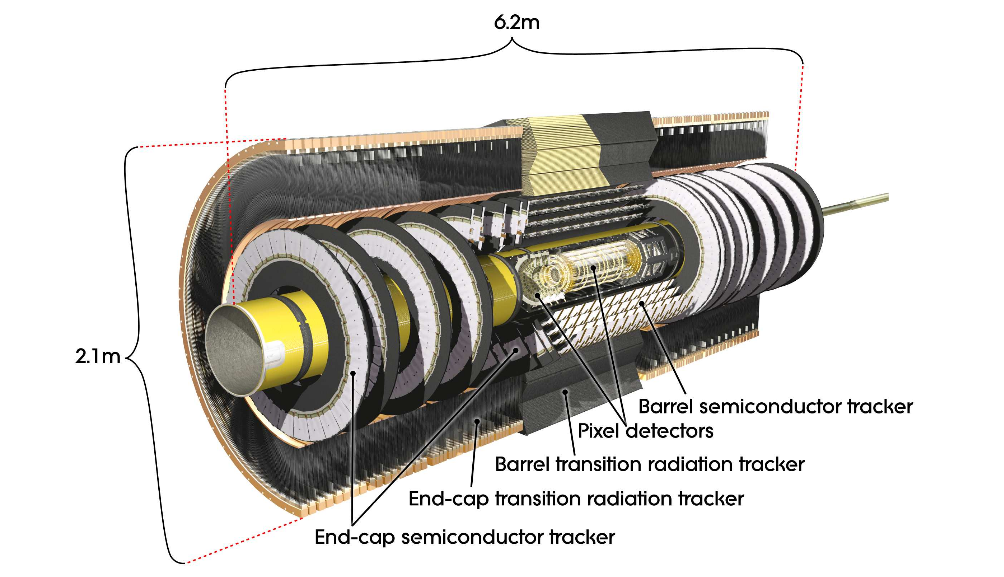
\includegraphics[width = \textwidth]{Figures/FromOnline/innerdetector.png}
    \caption{An illustration of the inner detector \cite{innerdetector}.}
    \label{fig:innerdet}
\end{figure}


\begin{figure}[H]
    \centering
    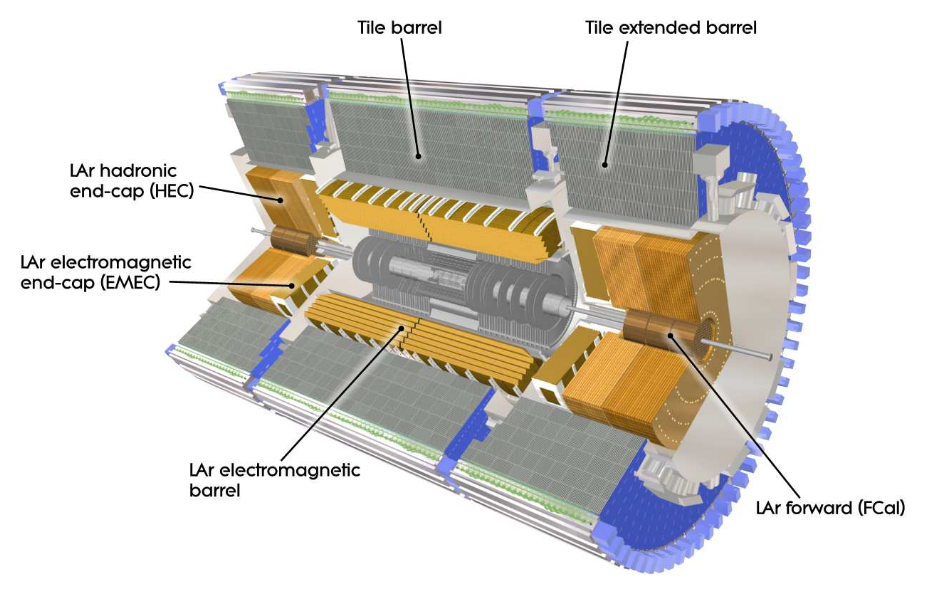
\includegraphics[width = \textwidth]{Figures/FromOnline/calorimeters.png}
    \caption{An illustration of the calorimeters \cite{innerdetector}.}
    \label{fig:calori}
\end{figure}


\begin{figure}[H]
    \centering
    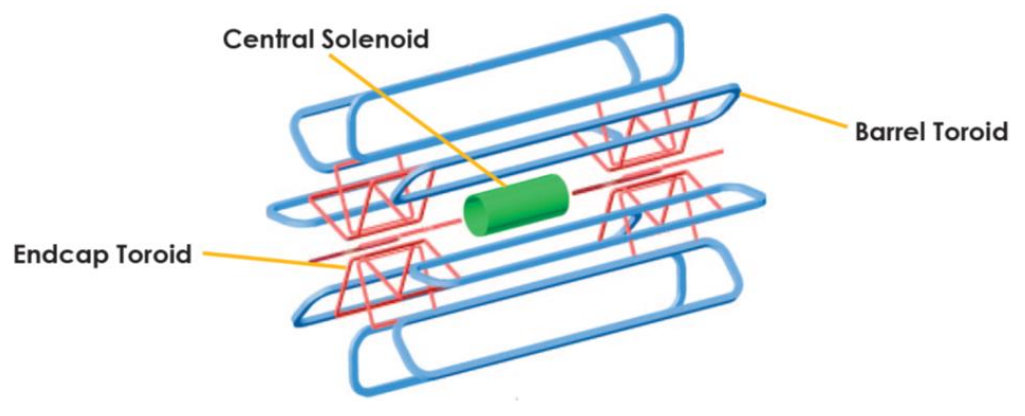
\includegraphics[width = \textwidth]{Figures/FromOnline/magnetsystem.png}
    \caption{An illustration of the magnet systems \cite{magnetsystem}.}
    \label{fig:magnetsys}
\end{figure}
\end{comment}



















\section{Computing infrastructure}
The results obtained in this thesis have been very comprehensive when it comes to computing power. It has not been possible to run the code on a regular computer because of not enough CPU's and memory. Because of these problems we have borrowed a server at Simula Research Laboratory, where we got to use the Experimental Infrastructure for Exploration of Exascale Computing. This is a computer with two sockets with 8 cores/CPU's, which again have two threads. This gives us in all 32 virtual CPU's (16 physical) because of hyper-threading in each CPU. It also have 60 GiB\footnote{GiB is Gibibyte instead of regular gigabyte and is simply a unit byte for digital information and means 2 to the power of 10 (kiB), 20 (MiB), 30 (GiB), 40 (TiB) and 50 (PiB).} memory, which have been crucial to handle the data used in ML. With this setup, the import of the data, training and testing have taken approximately 12-13 days, where 7 of these are just for importing the data. All together we have trained and tested 72 ML models (36 BDTs and 36 NNs) and the data sets we have been working on have been massive, where the memory have come in handy. 

In the final run-up of this thesis we have used a server that is in possession of the HEPP-group at UiO. It is a Supermicro Ultra Server with both GPU's and CPU's, but we have only taken advantage of the CPU's in this thesis. This server is a much more powerful computer than the one borrowed at Simula. It has two sockets with 128 cores/CPU's, which also have two threads in each CPU. This gives us a total of 256 virtual CPU's. It also has 2 TiB memory, which has resulted in that we could import the data in several parts and be done in around 3 days instead of a week. And we have been able to train around 18-20 ML models at the same time instead of 1-2 which was the maximum for the Simula server. 